\subsection{Processor}

The processor is modeled very similar to the design of the simple MIPS processor 
presented in Chapter 4.4 of the book Computer Organization and Design \cite{curriculum}. 
The largest change is that the instruction and data memory is not internal in the processor.
 The communication with memory is done through the ports of the processor. This relates to 
Figure 3.2 from the compendium \cite{compendium}. 

\begin{figure}[h]
	\centerline{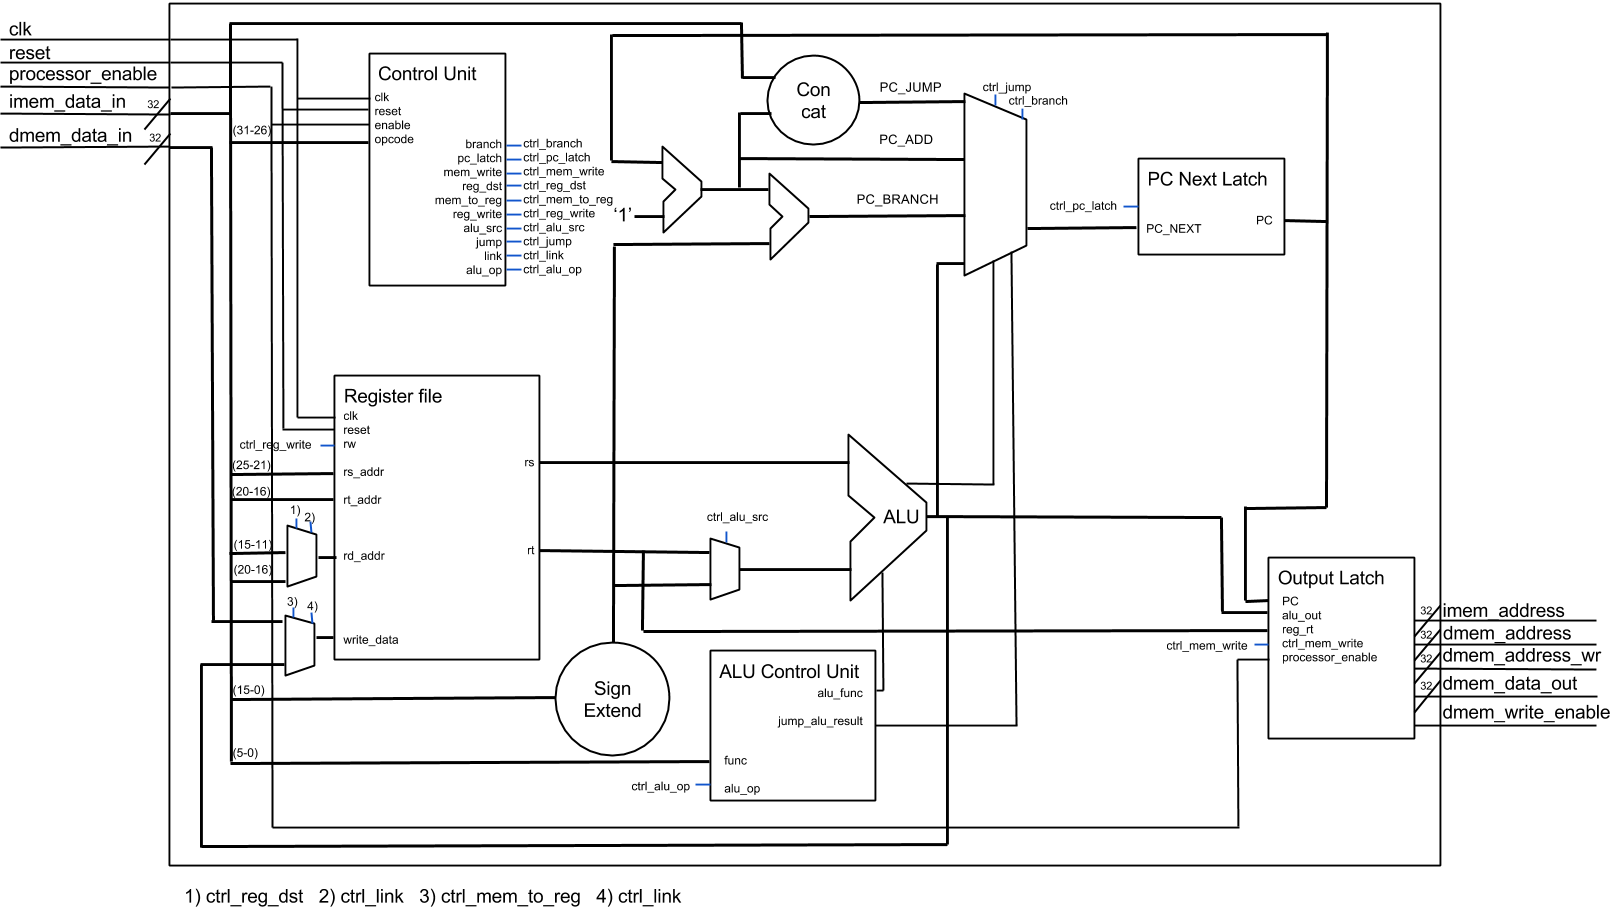
\includegraphics[width=550px]{figures/processor.png}}
	\caption{Processor}
	\label{fig:processor}
\end{figure}

The implementation of the processor is located in the processor.vhd file. Its outline is 
shown in figure \ref{fig:processor}. Here the core 
components of the processor, including the ALU, register file, control unit and alu control 
unit, are connected to each other. The components to take note of in this module are 
the muxes and latches. The rest are simple wiring. 

\subsubsection{Program Counter}
The Program Counter is represented by the PC signal. It is connected to the imem\_address 
output bus and is incremented by 1 word each cycle. The usual MIPS PC is defined to be 
incremented by 4 bytes each cycle, but given the fact that the memory module in this 
assignment addresses words instead of bytes, the PC is incremented by 1. Logic exists 
in this module to perform jump and branch instructions. 

\paragraph{pc\_mux} This mux lets the processor implement the different types of jump 
and branch instructions. It sets the PC\_NEXT signal to either alu\_out, PC\_JUMP, PC\_BRANCH or PC\_ADD. 

\paragraph{next\_pc\_latch} This latch enables the control unit to make sure that the PC 
is not incremented before the processor reaches the state FETCH in the start of each cycle. 

\subsubsection{Managing the register file}

This is where our extra feature jump and link comes in to play in the design. If the instruction 
{\bf jal} is executed the address PC+1\footnote{The MIPS specification states PC+8, but as the processor 
is not pipelined the branch delay slot was not implemented.} should be saved into r31.

\paragraph{req\_write\_mux} This mux multiplexes the different inputs for which register to write to. 
Possible sources are rt and rd parts of the instruction and LINK\_REG used by the jal instruction. 

\paragraph{data\_write\_mux} This mux is responsible for choosing the correct input to write to the 
register selected by the previous described mux. It selects the dmem\_data\_in bus for store instructions 
and otherwise it's set to the output of the ALU. The exception is the extra feature when the PC\_ADD signal 
is stored in the LINK\_REG for the Jump And Link instruction.

\subsubsection{Driving the outputs}

\paragraph{drive\_output\_signals} This latch prevents the processor from driving its 
output signals when processor\_enable is not asserted. 

\subsubsection{Control Signals}

The control unit outputs 10 different control signals. Each of these signals are connected to a component and alters either the datapath
or how the PC changes before the next instruction. The {\bf ctrl\_jump} and {\bf ctrl\_branch} is connected to the {\bf pc\_mux} and 
affects what value the next PC is given. The {\bf ctrl\_pc\_latch} drives the {\bf next\_pc\_latch} to tell it when to latch the pc. 
The manipulation of the common datapath is done by most of the signals. The register file is controled with {\bf ctrl\_mem\_to\_reg}, 
used for load instructions, {\bf ctrl\_reg\_dst} chooses the part of the instruction used to address the write in the register file, 
{\bf ctrl\_req\_write} whether or not to write at all. The {\bf ctr\_alu\_op} sets up the ALU with aid of the ALU Control Unit, this
signal can have one of the following values ALUOP\_LOAD\_STORE, ALUOP\_BRANCH, ALUOP\_FUNC, ALUOP\_LDI, refer to section \ref{sec:alu_control} for additional information.
{\bf ctrl\_alu\_src} controls a mux choosing either the rt output from the register file or the sign extended version of the 16 high
bits of the instruction. This configuration is used for jump instructions. Lastly in the datapath the {\bf ctrl\_mem\_write} lets the
processor enable output on the bus connected to data memory. The final signal called {\bf ctrl\_link} implements the extra feature. 
It is asserted when the {\bf jal} instruction is executed. This causes the muxes on the write address and data bus to set their values
to register \$31 and PC+1. This results in the next instruction address being saved in the link register.
